\documentclass{article}
\usepackage[margin=1in]{geometry}
\usepackage{graphicx}
\usepackage{hyperref}
\usepackage{natbib}
\usepackage{soul}
\usepackage{setspace} 
\doublespacing 
\usepackage{lineno} 
\linenumbers
\bibliographystyle{plain}

\title{Quantitative, Multispecies Monitoring at a Continental Scale}

\author{Gledis Guri$^1$\textbf{*} \and
Owen Liu$^2$ \and
Ryan P. Kelly$^1$ \and
Megan R. Shaffer$^1$\and
Kim Parsons$^2$ \and
Ana Ram\'on-Laca$^{1,2,3}$ \and
Krista M. Nichols$^2$ \and
Pedro F. P. Brandão-Dias$^1$ \and
Abigail Wells$^2$ \and
Andrew Olaf Shelton$^2$ \and}

\date{\today}

\begin{document}

\maketitle

\section*{}

\begin{center}
\begin{tabular}{ll}
1 & School of Marine and Environmental Affairs, University of Washington, Seattle, Washington, USA \\
2 & Conservation Biology Division, Northwest Fisheries Science Center,  NOAA Fisheries, \\
 & \qquad 2715 Montlake Blvd E. Seattle, Washington, USA \\
3 & Museo Nacional de Ciencias Naturales, Madrid, Spain \\
\hline
\textbf{*} & \textbf{Gledis Guri}, lead and corresponding author \textbf{gguri@uw.edu}
\end{tabular}
\end{center}

\section*{Significance statement}
Detailed information about living resources is often legally required to support management decisions, but the cost and difficulty of acquiring this information increases dramatically at large spatial scales. We present a scaleable, quantitative method for mapping genetic trace material from species of management interest, and use it to illustrate three-dimensional patterns of environmental DNA (eDNA) from fish species along the West Coast of the United States. The same technique is applicable to environmental samples of any kind and any number of species, and is therefore likely to be broadly useful in natural-resources management and in the life sciences more generally.

\section*{Author Contributions}
AOS, KMN, RPK, MS, and KP designed the research;\\
MRS, AR-L and AW did the laboratory work; \\
PB, RPK, and GG did the bioinformatics;\\
GG, OL, RPK, and eAOS analyzed the data;\\
GG, OL, RPK, and AOS interpreted the results;\\
All authors provided edits to the manuscript \\
Please check that this is correct and add/edit as needed XXX

\section*{Author Declaration}
The authors declare no competing interest.

\section*{Keywords}
eDNA $|$ Bayesian $|$ bio-monitoring $|$ quantification $|$ fish

\section*{Abstract}
Molecular data from environmental samples can reflect the abundance of species’ DNA, an index immediately relevant to natural-resources management at a broad geographic scale. These data commonly derive from assays designed and targeted for specific species (e.g., using qPCR or dPCR), or metabarcoding assays from more general PCR primers that amplify many species simultaneously. Multispecies analyses make efficient use of field samples and laboratory time, and speak to inherently multispecies questions of management and ecological research. However, unlike single-species techniques, metabarcoding by itself can reflect only the proportions of target-species DNA present, not their absolute quantities. Here, we combine qPCR and metabarcoding data derived from the same samples to map quantities of many fish species along the US West Coast in three dimensions, demonstrating a technique of practical importance for both management and ecology. We derive spatially explicit estimates of eDNA abundance for 12 common species of ecological and management importance and point the way to quantitative surveys of wild species using molecules alone. We find that species distribution maps derived from eDNA effectively capture species niches and spatial distributions. Notably, our analyses identified biodiversity hotspots that align with previously documented regions of ecological significance, such as the Columbia River plume and the Heceta Bank.


\section*{Introduction}
Environmental DNA (eDNA, residual genetic material sampled from water, soil, or air) is an increasingly common tool for non-invasively sampling marine and aquatic ecological communities, valuable for estimating species occurrence \cite{veilleux2021}, biodiversity (i.e., Richness, \cite{muenzel2024}), and genetic structure \cite{andres2023a}. However, eDNA has not been widely used for quantitative abundance estimation, upon which many practical management and conservation applications rely (but see \cite{shelton2022,guri2024a,stoeckle2022a}). The use of eDNA for quantification is supported both conceptually -- where there is more of a species, more cells are shed in the environment, and thus there is more DNA -- and empirically (e.g. there are strong linkages between single-species eDNA measures of in aquaria \cite{jo2019b,ledger2024}, rivers and streams \cite{pont2024}, estuaries and nearshore habitats \cite{dibattista2022, baetscher2024}, and coastal oceans \cite{maes2023, shelton2019}). However, uses of quantitative eDNA observations in management applications have significantly lagged behind their use in occurrence and biodiversity applications. 

Quantitative estimates of DNA are more common with species-specific assays (e.g. qPCR and ddPCR) because these approaches directly measure DNA concentration. In contrast, multispecies analysis (metabarcoding) reflects information on many species of interest simultaneously, but at the costs of producing compositional estimates of proportional abundance \cite{gloor2017a, mclaren2019} that may require statistical correction for species-specific biases due to PCR amplification \cite{shelton2023}. Consequently, metabarcoding data alone cannot yield information about the abundance of DNA from environmental samples (e.g. \cite{guri2024a}).

While trawling and other traditional sampling methods have been the fundamental tools for directly measuring fish abundance and biomass, they are often impractical for species inhabiting inaccessible habitats, occurring at low densities, or fragile species easily injured during capture. By contrast, eDNA sampling captures information on a broader range of taxa, including those that are difficult or impossible to study with traditional gear. As such, eDNA can meaningfully complement traditional stock assessment methods for commercially important species while at the same time revealing the abundance and distribution of elusive or understudied species.

Here, we develop quantitative estimates of eDNA abundance for a diverse group of fish species spanning different depth niches across 10 degrees of latitude along the US West Coast entirely from eDNA. We integrate single- and multi-species (using MiFish-U universal primers \cite{miya2015}) techniques to create three-dimensional distribution maps, leveraging models established in previous studies \cite{shelton2022, guri2024a, shelton2023, allan2023}. By calibrating metabarcoding data -- correcting raw species observations to their initial proportions using a mock community \cite{shelton2023} -- and using the absolute eDNA quantity of a reference species (here Pacific Hake (\textit{Merluccius productus})), we expand initial estimated proportions into absolute estimates of the abundance of each species’ eDNA \cite{guri2024a}. We subsequently smooth the estimated eDNA quantities to generate species distribution maps \cite{liu2023}. We present results for 12 fish species to illustrate the approach, but note that it immediately generalizes to any ecological community of interest.

The eDNA-derived estimates we provide here speak directly to the requirements of natural-resources management at large scales. For example, indices of abundance have a central role in determining stock status for fisheries applications (i.e., stock assessments in the U.S. under the Magnuson-Stevens Act) as well as informing conservation status (e.g., under the U.S. Endangered Species Act). Thus eDNA-derived abundance indices can fill a variety of existing requirements for management. While these indices are still in their infancy and will require additional technical developments to ensure their proper usage, they are conceptually and practically little different from abundance estimates derived from more traditional ocean survey methods (i.e., net-based or acoustic surveys). Indeed, eDNA methods may provide some notable improvements because single- and multi-species eDNA approaches avoid tradeoffs involved with physically capturing many species simultaneously using a single net. Molecular surveys capture many species with the same ``gear" using methods that are easily replicated in space and time. As U.S. agencies begin to implement the new National Aquatic eDNA Strategy \cite{kelly2024} -- the first goal of which is to fold eDNA data into federal decisionmaking -- this and other large-scale examples point the way to maximizing the benefit of this information-rich datastream for natural-resources management at a continental scale.

\section*{Results}
We find spatial patterns of DNA concentrations reflect the distributions of commercially important coastal-pelagic fish species in three dimensions and across ten degrees of latitude in a single year of sampling in 2019 (Fig. \ref{fig:fig1}: Northern Anchovy, Pacific Sardine; \href{SI_Appendix.pdf}{SI Appendix, Fig. S1}, Pacific Herring and Jack Mackerel). For other high-biomass species otherwise lacking well-described distributions, we provide the first species distribution models (Fig. \ref{fig:fig1}, \href{SI_Appendix.pdf}{SI Appendix, Fig. S1}). We find that the estimated eDNA concentrations are correlated among species with similar traits and habitat preferences (Fig. \ref{fig:fig2}). Emergent patterns of species richness and estimated eDNA aggregation correspond with known ecological drivers, evidence that eDNA traces can reliably capture ecologically meaningful patterns (Fig. \ref{fig:fig3}). Particularly for forage fish species – which are critical high-biomass links in marine food webs, but difficult to survey with traditional methods \cite{Pikitch2012} – molecular methods offer a tractable and quantitative index of abundance over large spatial scales.

Below we highlight results for six species (Fig. \ref{fig:fig1}) representing a range of habitat associations and general species information; distribution maps for all the remaining species are presented in \href{SI_Appendix.pdf}{SI Appendix, Fig. S1}.

\begin{figure*}[tbhp]
\centering
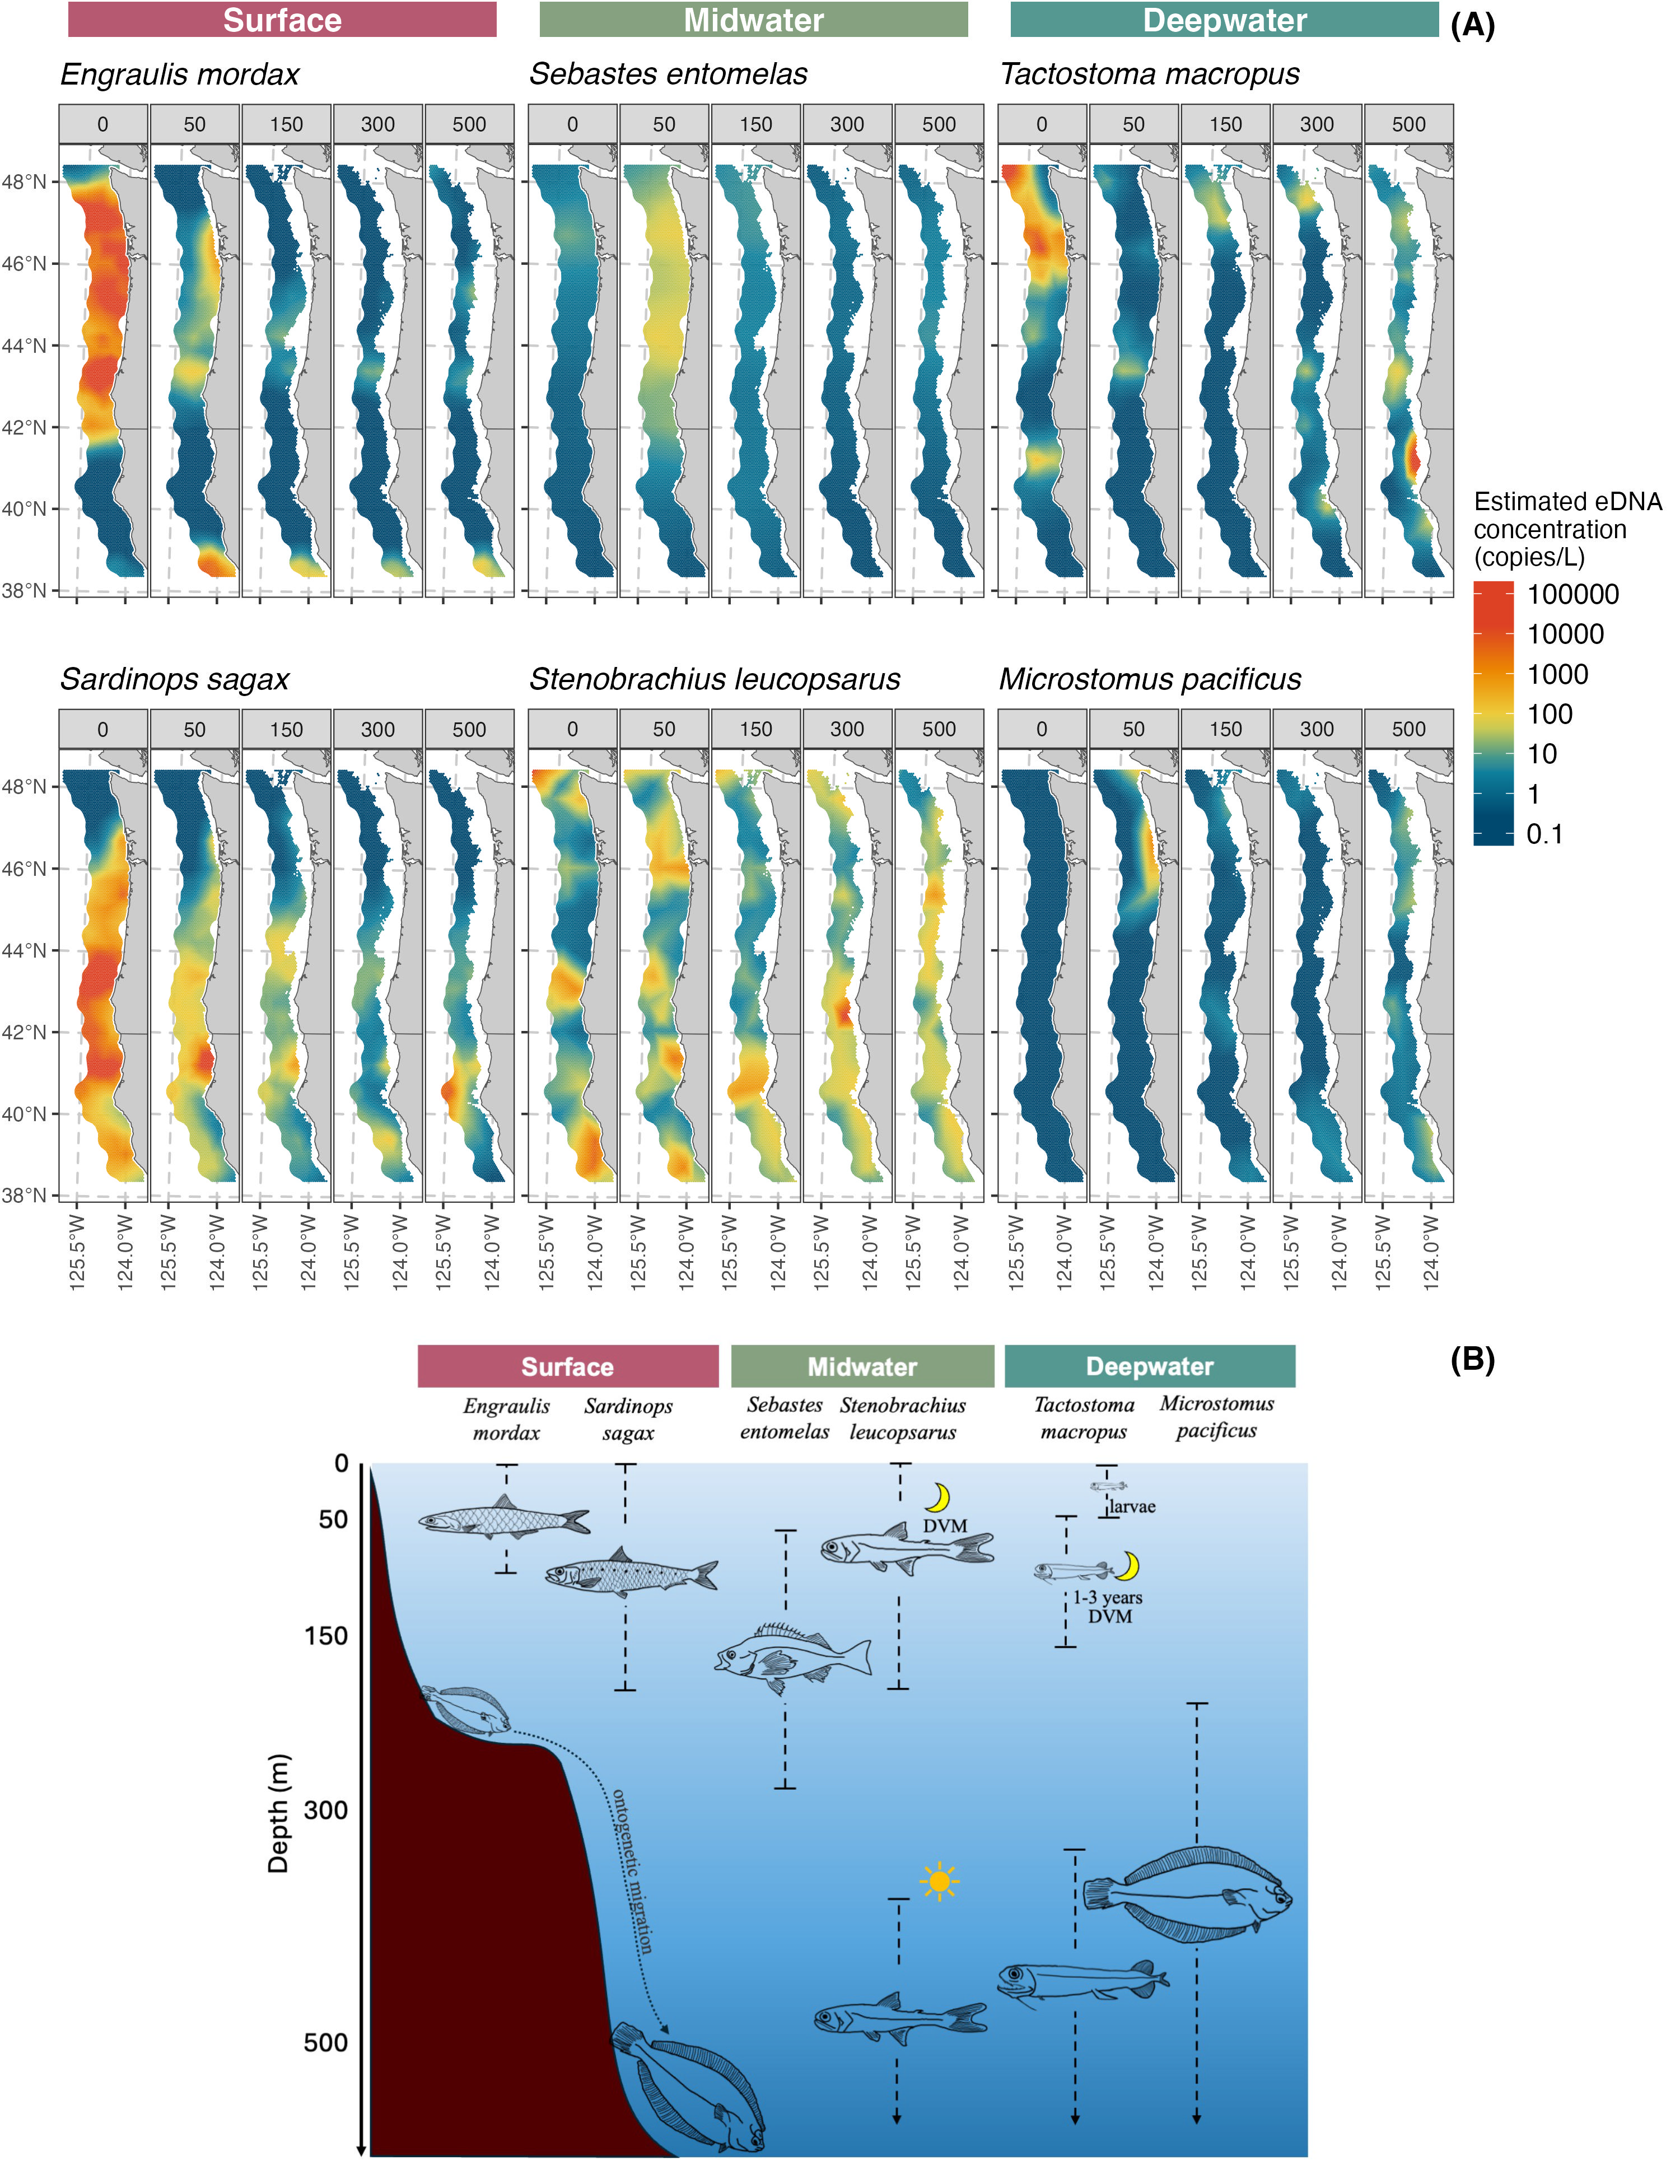
\includegraphics[width=16cm]{plots/1_Figure_1.jpg}  % Adjust width to 11.4 cm or 17.8 cm as per the template
\caption{Estimated species eDNA concentration (A) across 0, 50, 150, 300, and 500m depth samples and known depth distribution of those species from literature (B).}
\label{fig:fig1}
\end{figure*}

\subsection*{Surface}
Northern anchovy (\textit{Engraulis mordax}) and Pacific sardine (\textit{Sardinops sagax}) are the two iconic coastal pelagic species of the eastern North Pacfic \cite{steinbeck1945} and play a vital ecological role linking lower and upper trophic levels (e.g., Chinook salmon diets, sea lions, \cite{kaplan2019}); historically these supported large commercial fisheries particularly in California. Our eDNA estimates consistently reflect the expected three-dimensional distributions of each species, with high concentrations in surface waters for both species at northern latitudes \cite{litz2008,parnel2008} particularly near the Columbia River outflow (46.2°N; Fig. \ref{fig:fig1}). Sardine favors slightly warmer temperatures and more southerly waters than anchovy (SST range from literature: 13–24°C for sardine vs. 10–14°C for anchovy).  We found more Pacific sardine DNA in sub-surface waters as well (Fig. \ref{fig:fig1}). eDNA patterns tracked these differences with sardine eDNA in greatest abundance at 41°N (range 40°–45°), while anchovy eDNA abundance was greatest at 43.5°N (range 42°–48°; Fig. \ref{fig:fig4}) such that eDNA captured subtle yet meaningful differences in habitat preferences. Furthermore, eDNA abundance patterns suggest a 2.5-fold higher abundance for anchovy than sardine which agree in direction with stock assessments for anchovy and sardine (an approximately 35-fold difference; \cite{kuriyama2022, kuriyama2022b}). However, due to differences in stock definitions and survey areas (the anchovy stock assessment includes southern California waters (32.5°–36° N) not covered by the eDNA survey) these magnitudes are not directly comparable.

\subsection*{Mid-water}
Widow rockfish (\textit{Sebastes entomelas}) is common between 100-350m between northern Baja California and southern Alaska, with pelagic larvae and juveniles generally detected in shallower habitats ($<$ 150m depth) \cite{reynolds2001,bosley2014} including in nearshore kelp forests \cite{quigley2024, laidig2007} . Moreover, because it is a common bycatch species in the Pacific hake (\textit{Merluccius productus}) fishery, concerns about bycatch of widow rockfish can also influence the much larger hake fishery (i.e., it is a “choke” species for hake; \cite{somers2018}). Despite its commercial importance, no targeted survey effort exists for widow rockfish, in part because bottom trawls do not sample its pelagic habitat well. We find widow rockfish eDNA strongly and nearly exclusively associated with 50m sample depths (Fig. \ref{fig:fig1} and \ref{fig:fig4}), consistent with the pelagic larvae and juveniles reported in the literature and somewhat shallower than adults are commonly found \cite{reynolds2001,bosley2014,quigley2024}, potentially reflecting the species’ nocturnal feeding schooling behavior \cite{reynolds2001,bosley2014}.

The eDNA patterns for northern lampfish (\textit{Stenobrachius leucopsarus}) -- an abundant myctophid that migrates from 400-700m up to 20-200m at night \cite{moku2000,suntsov2008} -- are again consistent with the ecology of the species, having notably lower concentrations in surface samples. Owing to the diel vertical migration of the northern lampfish, the signal of eDNA for this species is observed across depths.

\subsection*{Benthic}
Among deeper-water fishes, eDNA revealed spatial and potentially ontogenetic migration patterns for species that are common, yet under studied, such as the dragonfish (\textit{Tactostoma macropus}). Available literature suggests dragonfish occur roughly between 40°N-50°N (adults at 300-900m, larvae at 0-60m in summer) \cite{kawaguchi1993} and perform diel vertical migrations to around 100 meters \cite{kawaguchi1993,willis1982}. The eDNA concentrations appeared to reflect this activity (Fig. \ref{fig:fig4}), with the predominant surface signal at northern latitudes likely reflecting larvae and juveniles (Fig. \ref{fig:fig1}), and two deeper hotspots at 300m and 500m separated by about eight degrees of latitude. However, no other quantitative estimates of abundance or detailed distribution patterns for dragonfish exist in the current literature.

Also consistent with known habitats are commercially caught flatfish such as Dover sole (\textit{Microstomus pacificus}), which lives at 200m to 1200m along the Pacific coast \cite{drazen2007,brodziak2000,drazen2012}; individuals move progressively deeper as they grow \cite{vetter1994,hunter1990}. The eDNA concentration estimates are consistent with this pattern, showing high concentrations mostly in water samples collected close to the seabed (Fig. \ref{fig:fig4}\textit{A}) \cite{ono2016}.

\subsection*{Species Associations}

Pairwise correlations of DNA concentration showed interesting patterns among species associated with depth (Fig. \ref{fig:fig2}). Surface-associated species were nearly all positively correlated with each other, with some correlations particularly large (Pearson's $\rho > 0.50$). Correlations were weak among the six midwater and deepwater species (all $\rho < |0.40|$). Within the surface species, further subdivision was also apparent, with chub mackerel (\textit{Scomber japonicus}) and sardine (\textit{Sardinops sagax}) showing very high correlation ($\rho = 0.76$) with both more common in the more southern (and somewhat warmer) waters (Fig. \ref{fig:fig1} and Fig. \ref{fig:fig4}). Concentrations of the remaining surface-dwelling species (Northern anchovy, eulachon, jack mackerel, and Pacific herring) had modest correlations with midwater species (Fig. \ref{fig:fig2}) consistent with more northerly distribution (Fig. \ref{fig:fig4}). Together these finding suggest that eDNA is capturing both depth and latitudinal habitats associations. Deep-water species are distinct (Fig. \ref{fig:fig1} and Fig. \ref{fig:fig4}) and not strongly correlated with those from other zones (Fig. \ref{fig:fig2}). Deeper water tends to feature lower and more diffuse fish eDNA concentrations (Fig. \ref{fig:fig1} and Fig. \ref{fig:fig4}). Lower overall eDNA concentrations and fewer deep water samples may make similarities among species distributions more difficult to detect at 300m and deeper.

\begin{figure}[tbhp] 
\centering
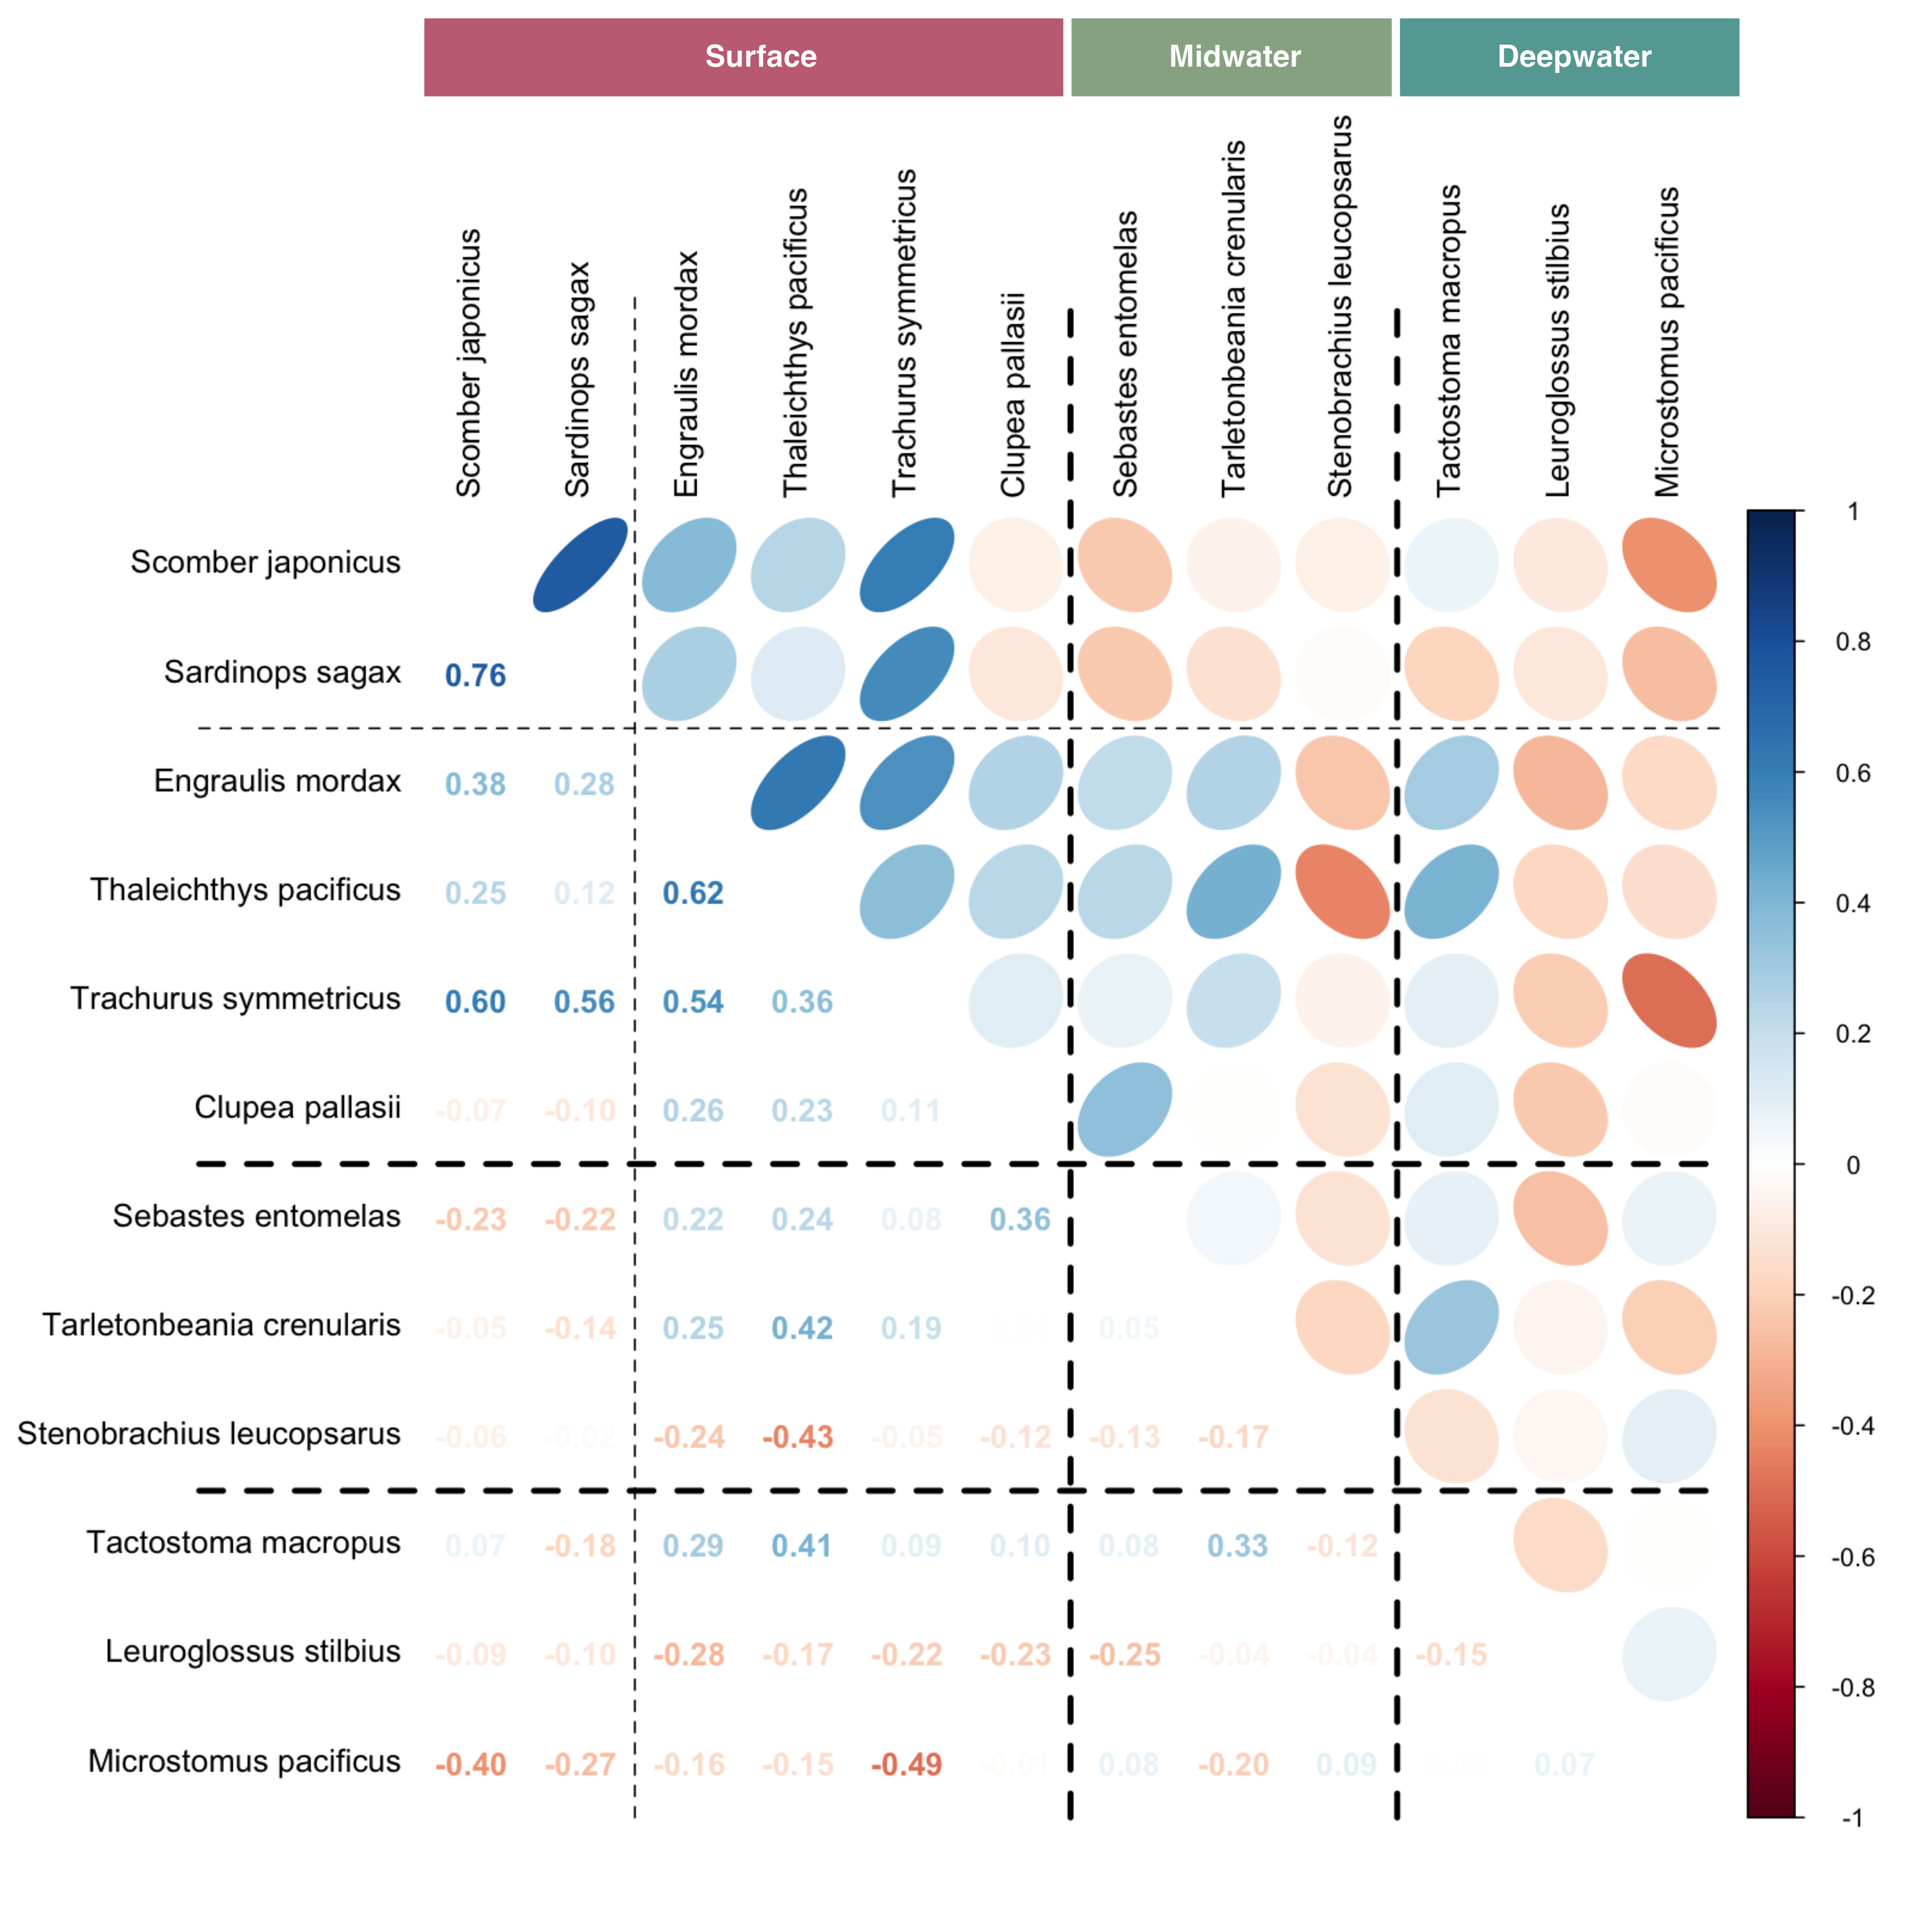
\includegraphics[width=10cm]{plots/2_Figure_2.jpg}  
\caption{Correlation plot describing species co-abundance and co-occurance. Spearman’s rho correlation coefficient are expressed in numbers and colors ranging from -1 (red) negatively correlated to 1 (blue) positively correlated. Species are ordered in known ecological groups (surface, midwater, and deepwater) to visually indicate the gradual change of species co-occurance.}
\label{fig:fig2}
\end{figure}

\subsection*{Species richness and total eDNA accumulation}
In addition to providing species-specific patterns, eDNA metrics of abundance from individual species can be combined to reveal important aggregate ecological patterns. For the 12 species considered here, we show how species richness (see \href{SI_Appendix.pdf}{SI Appendix Fig. S3} for defining species presence) from eDNA varied substantially and predictably with depth, with the highest richness observed at the surface (Fig. \ref{fig:fig3}\textit{A}). In part, this pattern is likely to be an artifact of the focal species included in this study -- chosen for their relevance to fisheries management as well as for their frequency in the observations (see Methods) -- but the richness-depth gradient also reflects the expectation that habitat and nutrient availability is greatest near the surface \cite{smith2002,hickey2005}. Surface waters also host the eggs, larvae, and juvenile stages of many meso- and bathypelagic species \cite{parnel2008}, some of which we detect, and hence we both expect and observe higher richness in the upper layer of the water column \cite{kim2011}.

Species richness also corresponds strongly with the influence of Columbia River plume (Fig. \ref{fig:fig3}\textit{A}), which extends well beyond the coastline \cite{hickey2003}. The nitrate-rich river water interacts with ocean currents and intensifies coastal upwelling, enhancing both primary and secondary productivity \cite{hickey2010} and likely influencing the patterns of species richness we observe (Fig. \ref{fig:fig3}\textit{A}) \cite{tolimieri2015}. The total fish eDNA accumulation (Fig. \ref{fig:fig3}\textit{B}) suggests the highest aggregation of forage fish DNA near Heceta Bank (44 degrees N; overlapping anchovy and sardine distributions are the two largest contributors to eDNA concentration) in addition to other commercialy important mesopelagic fish (\textit{Sebastes entomelas} and \textit{Tarletonbeania crenularis}) a center of abundance for commercial fisheries \cite{bosley2014,Tissot2008TwentyYO}, and elsewhere nearshore in areas of coastal upwelling.

\begin{figure*}[tbhp]  
\centering
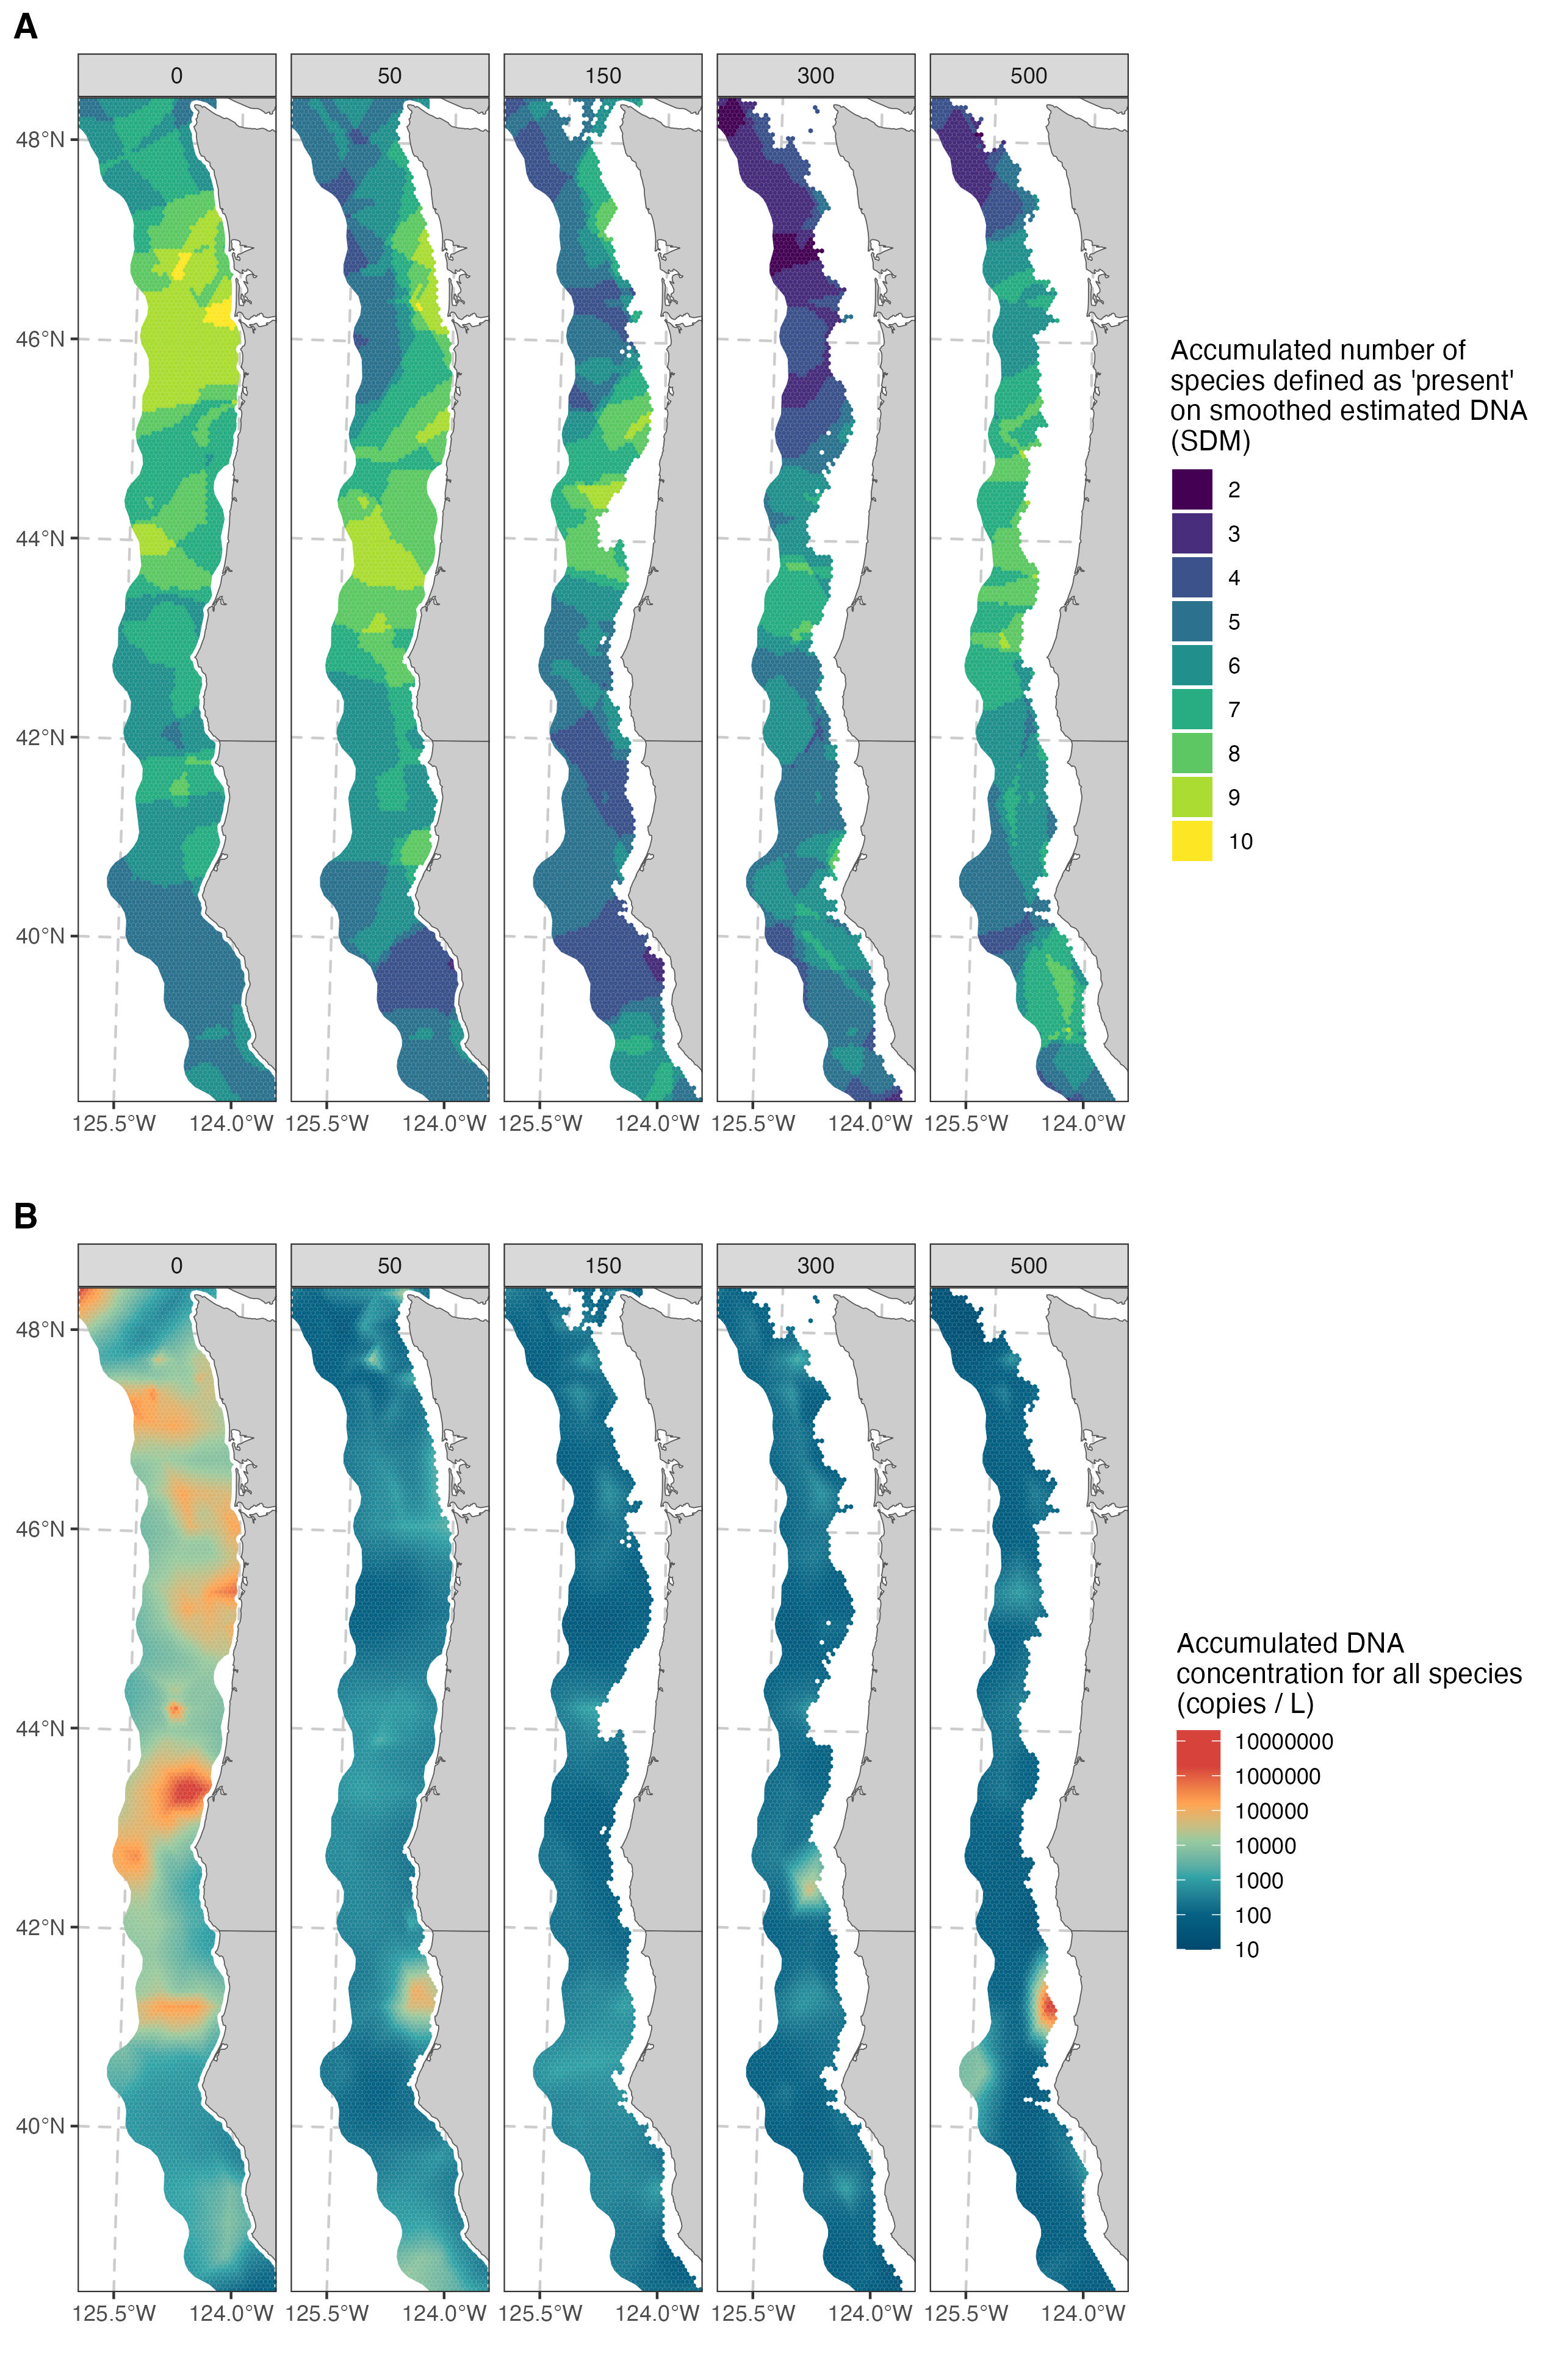
\includegraphics[width=13cm]{plots/3_Figure_3.jpg}  
\caption{Spatial and vertical distribution of species richness (A) and environmental DNA (B) concentration across depths (0, 50, 150, 300, and 500 m). (B) Species richness represented as the cumulative number of species present (species with higher than 1.5 copies/L (see Fig. \ref{fig:fig4} for defining presence) on smoothed estimated eDNA concentrations) and acumulated eDNA concentration representing the cumulative sum of eDNA (copies/L) across all species.}
\label{fig:fig3}
\end{figure*}

\begin{figure*}[tbhp]  
\centering
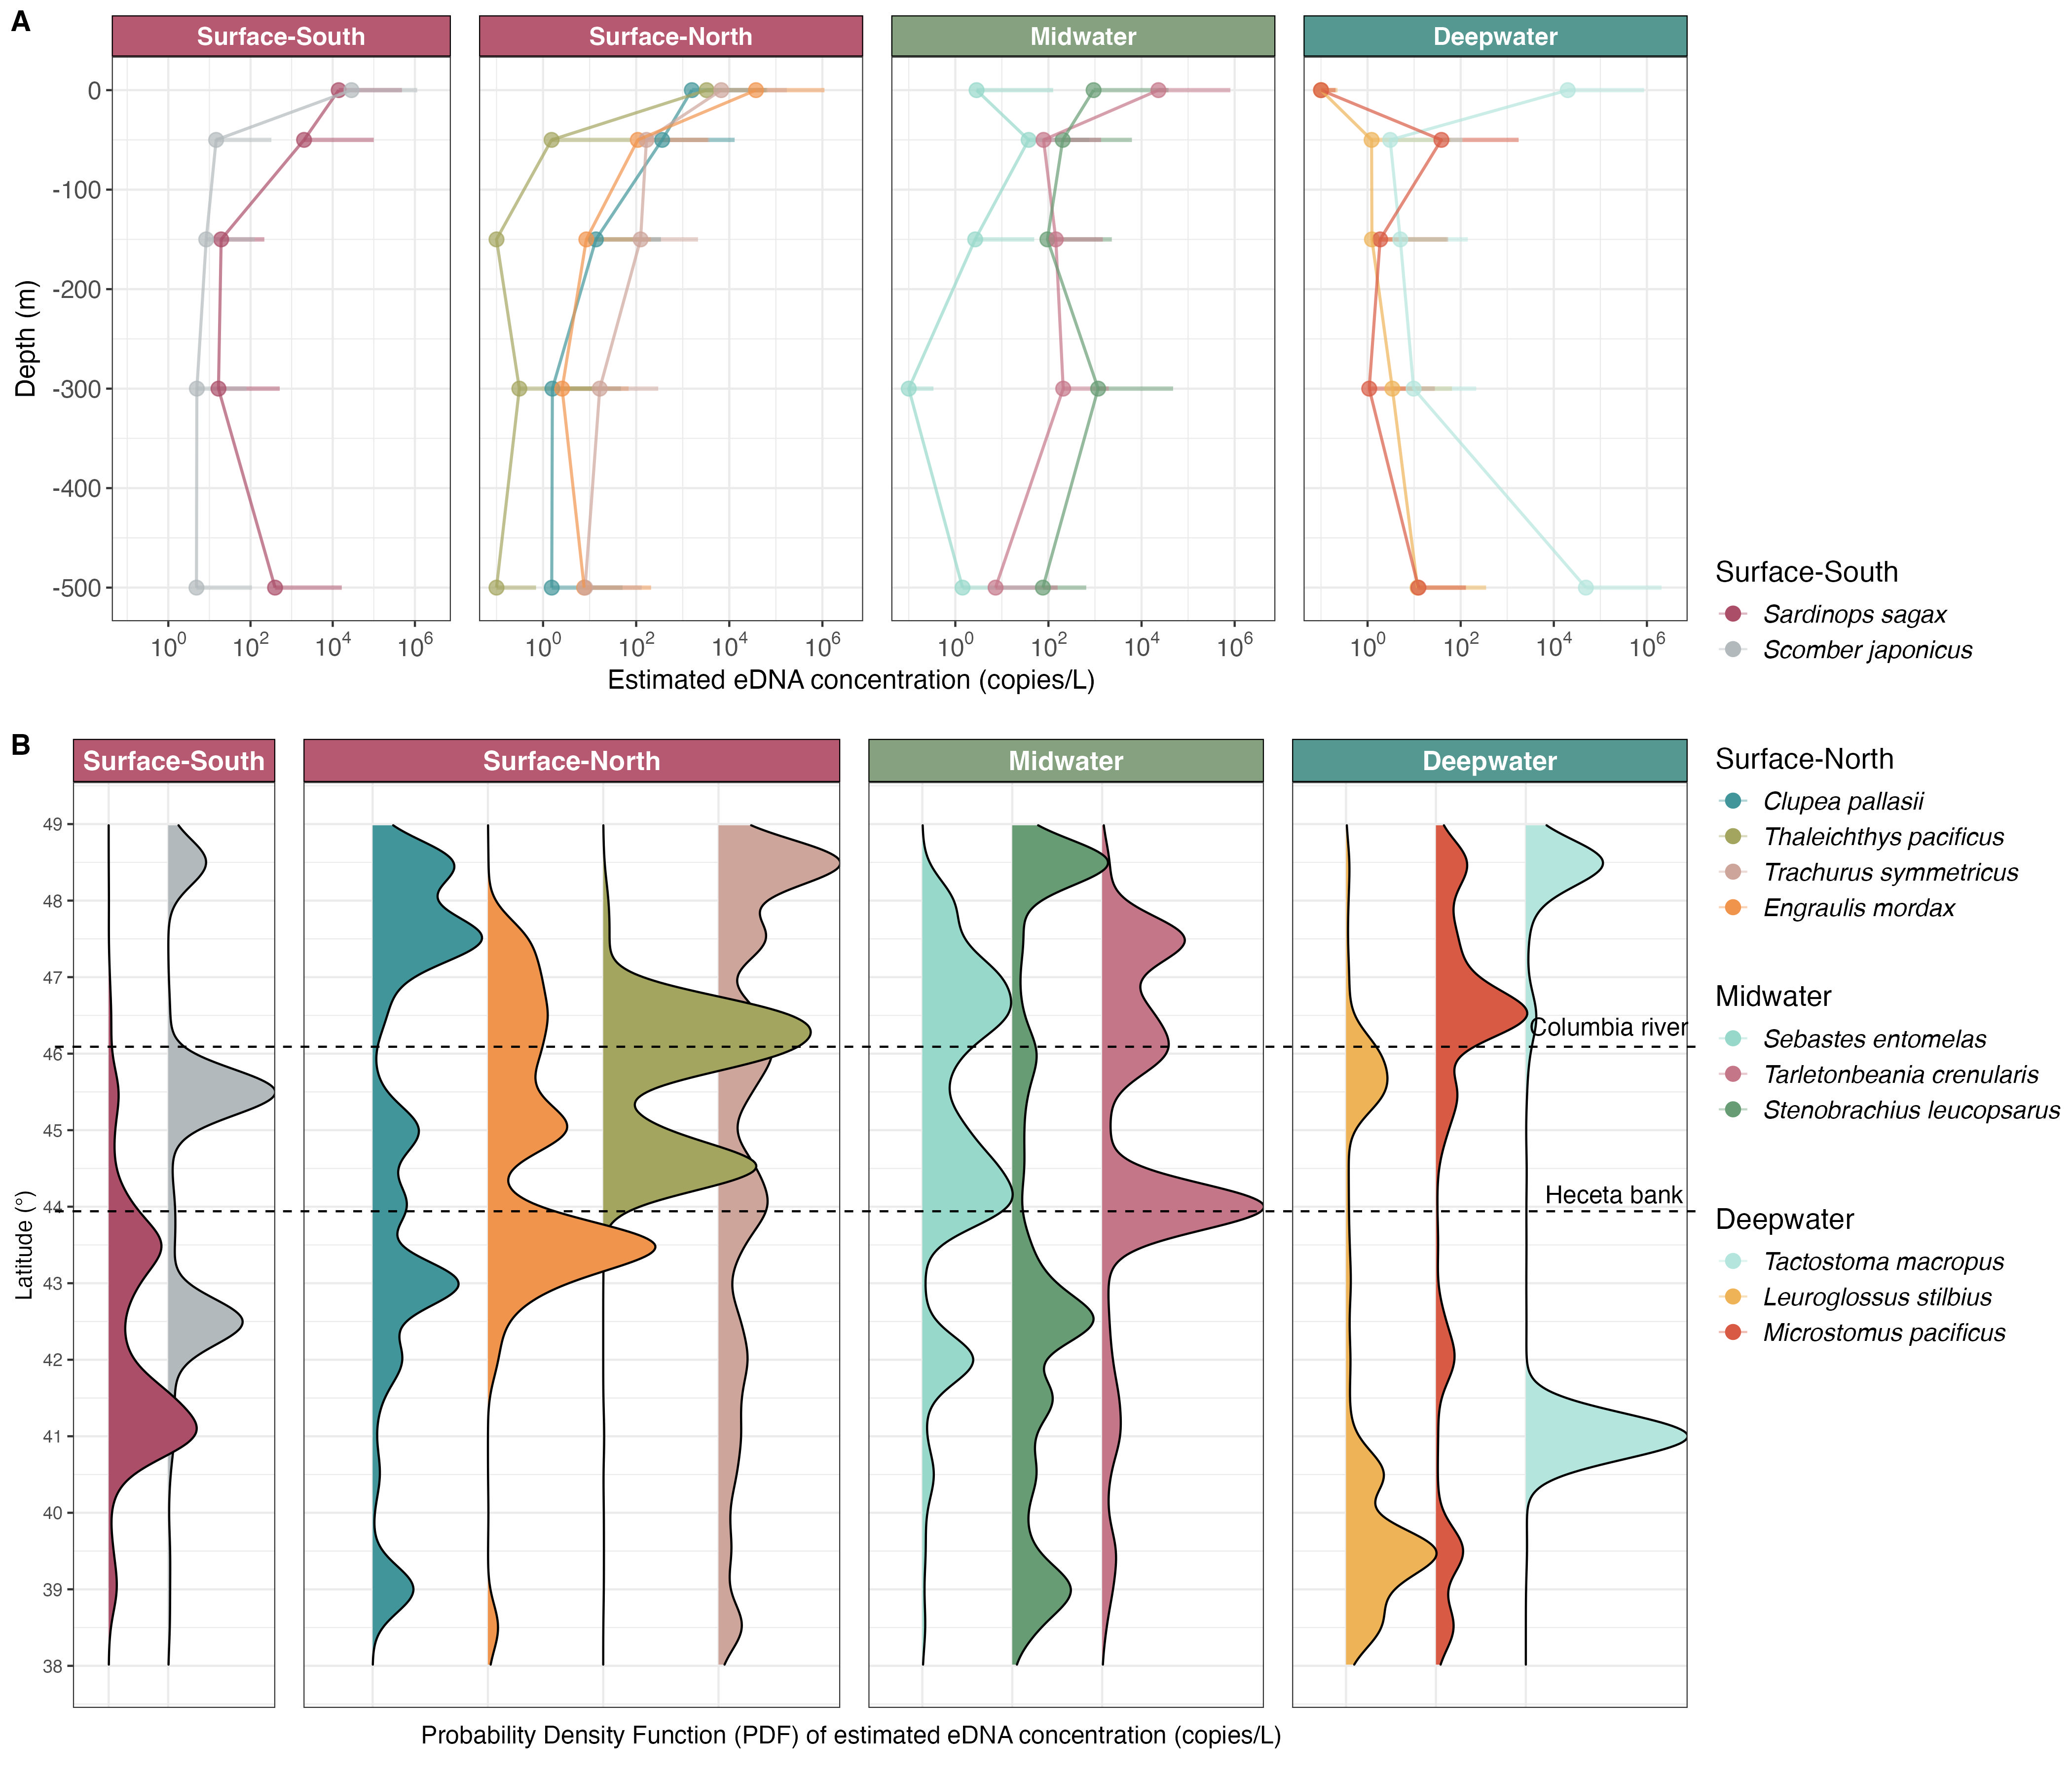
\includegraphics[width=17cm]{plots/4_Figure_4.jpg}  % Adjust width to 11.4 cm or 17.8 cm as per the template
\caption{Vertical (A) and latitudinal (B) distribution of eDNA concentrations grouped in ecological groups (surface south, surface north, midwater, and deepwater). Mean eDNA concentration of vertical distribution is shown with dots and 99\% upper quantile with ticks (A). Probability density functions (PDF) of estimated eDNA concentrations across latitudinal gradients (B; square root transformed of x-axis to enhance low concentration peaks). Key geographic features, such as the Columbia River and Heceta Bank, are marked to indicate alignment of species distributions.}
\label{fig:fig4}
\end{figure*}

\section*{Discussion}
We report species-specific DNA concentrations smoothed over ten degrees of latitude and across the continental shelf to 500m. We reveal distributional pattern for 12 species ranging from the iconic coastal pelagic species of the northeast Pacific to understudied-but-abundant deepwater species, and our results suggest clear pathways for the broader use of eDNA in both fisheries and ecosystem management.

\subsection*{eDNA as Management Tool}
By mapping three-dimensional spatial patterns, eDNA provides information on species distributions, habitat preferences, and ecological processes that is often otherwise unavailable. A single water sample can yield quantitative information on tens to hundreds of species -- including for species for which traditional fisheries surveys are not currently conducted -- without the need to develop species-specific assays. We find species-level eDNA concentrations align closely with the preferred habitats' physiological constraints (e.g., temperature tolerance or food availability) described for each species in the available literature. The observed latitudinal differences of eDNA concentration among species – such as those between anchovy and sardine – highlights species’ thermal ranges and largely coincide with other surveys \cite{zwolinski2024}; moreover, eDNA patterns appear to reflect diel vertical migrations as observed in myctophids, where eDNA concentrations are consistent with the species’ ontogenetic movement between surface and mid- to deep-water habitats. We also identify aggregations of richness and total eDNA near high-productivity regions of ecological and commercial value. Regions like Heceta Bank host dense aggregations of forage fish and are critical for both fishery management and for broader marine food-web stability. 

For well-studied taxa, existing information helps contextualize eDNA signals, providing insights into habitat preferences, seasonal patterns, or temperature tolerances. For poorly studied species, eDNA serves as an exploratory tool, detecting elusive taxa and revealing unexpected habitats. Widow rockfish, for example, appear almost exclusively in pelagic habitats around 50m deep, which are sampled poorly by traditional bottom-trawl surveys \cite{keller2017}. This species has been of special interest, as its targeted commercial harvest resumed in the late 2010s after a decade of closure (harvest was less than 500 mt annually between 2003 and 2013 but has exceeded 10,000 mt annually since 2018) and no existing survey adequately captures its patterns of abundance \cite{adams2019a}.

\subsection*{Environmental Smoothing}
Our findings underline eDNA as a transformative tool for fisheries management, biodiversity conservation, and the study of environmental change. However, the observable eDNA signal at any given location and time is an integrated product of DNA production and loss across time and space \cite{gold2023}: the vast majority of DNA detectable in a given sample is of recent origin (within the previous hours to days \cite{strickler2015,collins2018,machler2018}), and it may be subject to a degree of physical transport within its window of detectability. Accordingly, the vast majority of DNA will be relatively proximate to its source in both space and time, and the distribution of DNA from a given species at any given time will be smoother and more extensive when compared to the distribution of discrete source individuals. We refer to this as environmental smoothing of eDNA signal relative to the source organisms themselves. 

The majority of eDNA shed into the environment dissipates from surface waters within hours \cite{andruszkiewiczallan2021}. Thus, the horizontal scale of environmental smoothing in our dataset likely spans several kilometers at most \cite{baetscher2024}. Given that our sampling area spans more than 1,200 km north to south and tens of km east to west, the spatial patterns we report are likely to reflect genuine differences in fish communities rather than artifacts of eDNA transport dynamics \cite{guri2023}. Vertical smoothing of eDNA signals appears minimal, with patterns at the scale of meters: shallow-water species (sardine, anchovy, herring) occur largely at the surface and 50m depth bins; Widow rockfish occurs almost exclusively at the 50m depth; species found throughout the water column are either diel vertical migrators or species occupying different depths at various life-history stages (Fig. \ref{fig:fig3}\textit{B}); and bottom-dwelling fishes are detected primarily at the deepest point sampled on any station. 

Notably, the comparison between sample-specific eDNA estimation (\href{SI_Appendix.pdf}{SI Appendix, Fig. S6}) and spatially smoothed maps (Fig. \ref{fig:fig1} and \href{SI_Appendix.pdf}{SI Appendix, Fig. S1}) revealed minimal differences. Large-scale sampling combined with statistical smoothing mitigates many challenges associated with eDNA transport and degradation -- which decouple the eDNA observations from their particular source organisms -- allowing reliable detection of broad patterns in species distributions. Further methodological improvements may incorporate information about the ecology of eDNA itself, such as the degree to which observations of eDNA concentrations depend upon water temperature or other covariates \cite{jo2019b}. 

\subsection*{Integrating DNA with traditional surveys}
Effective management of natural resources at large scales requires that we maximize the information content of existing sampling regimes. Here, we follow \cite{shelton2022}, leveraging the same water samples to provide information on an additional 12 species of ecosystem and management importance. Elsewhere, a subset of these samples has yielded information on the distribution of marine mammals \cite{valdiviacarrillo2025}. The repeated use of a single set of samples highlights an important strength of eDNA samples; they allow researchers to revisit and re-sequence the genetic material in archived samples as new research questions arise or attention shifts to different taxa. The use of these samples, from a targeted fisheries survey for hake, highlights the efficiency for which eDNA can effectively provide survey data for tens or hundreds of additional species for which traditional surveys do not exist. 

This capacity for retrospective analysis allows historical samples to be re-examined at any point, insofar as the sample is not exhausted, thereby offering opportunities to address emerging priorities and to reconstruct past ecological conditions. For example, the ability to retrospectively pinpoint the origins and pathways of invasive species can inform targeted interventions, helping managers understand not only where an incursion began but also how it spread \cite{gilbey2021}. Similarly, the capacity to trace the initial onset of harmful algal blooms or the earliest presence of pathogenic microbes enables researchers and policymakers to identify the underlying drivers of these events and mitigate future outbreaks \cite{shaw2019}. 

Moreover, integrating retrospective eDNA analyses into climate change modeling can enrich predictive frameworks by providing historically grounded baselines of community composition, thereby enhancing our understanding of ecosystem responses to environmental shifts. For example, \cite{diaz2020} demonstrated how archived samples could be leveraged to reconstruct past fish communities using eDNA, thereby complementing traditional monitoring methods and further extending the utility of archived material. Such retrospective applications deepen and extend the value of every research expedition, ensuring that once-collected samples continue to yield valuable ecological insights over time. We therefore see eDNA as an important datastream that maximizes the information value of existing research cruises, rather than a means of replacing those cruises themselves.

We have shown an example of the substantial value of multi-species eDNA analysis for fisheries and other natural-resource management questions \cite{ledger2024,stoeckle2024}, however, molecular patterns alone are unlikely to drive quantitative natural-resources decisions, in part because eDNA generally does not provide auxiliary information important for managing populations (e.g., information on size- or age structure, fecundity, sex, or disease). Moreover, the eDNA sampling we describe here depends upon survey vessels that can reach and sample from deep water – survey vessels that exist to carry out traditional acoustic or trawl-based surveys. Furthermore, eDNA survey provide data in units of eDNA concentration, not more familiar units of mass or abundance. Relating observed eDNA concentrations to species mass requires data external to the eDNA signal \cite{guri2024a}, and in particular, requires that we understand proportionalities between eDNA concentration and biomass that may vary among species. We therefore see eDNA analysis as strengthening and extending existing surveys, with different data streams complementing one another. 

Conventional fish surveys, such as trawling or mark-recapture methods, typically rely on a closure assumption assuming that fish populations are static during the sampling period \cite{bailey2014}, ignoring the reality of fish movement within the study area thus introducing potential bias into abundance estimates \cite{rota2009}. By contrast, eDNA analysis leverages the continuous shedding of DNA by fish, which decays over time with higher concentrations remaining fresh while older DNA persists at lower levels \cite{thomsen2015,jerde2011}. This cumulative, time-integrated signal allows eDNA surveys to circumvent the closure assumption and provide a more accurate representation of fish presence and activity.

\section*{Methods}
We summarize all methodological components and provide details for all sampling, laboratory, and statistical methods in the \href{SI_Appendix.pdf}{SI Appendix Extended Methods}.

\subsection*{Sample Collection, Processing, and Quantitative PCR (qPCR)}
We used samples collected in 10L Niskin bottles deployed on a CTD rosette at six depths (0, 50, 150, 300, 500 m) from stations along the West Coast of the US aboard the ship \textit{Bell M. Shimada} during Summer 2019 on the Joint U.S.–Canada Integrated Ecosystem and Pacific Hake Acoustic-Trawl Survey \cite{deblois2020}. 2.5L water samples were collected from each Niskins and filtered immediately on 47 mm diameter mixed cellulose-ester sterile filters with a 1 $\mu$m pore size, subsequently extracted using a phase-lock phenol-chloroform protocol, and analyzed in triplicate using a qPCR assay, multiplexed for Pacific hake, sea lamprey, and eulachon, as described in \cite{ramon-laca2021} and \cite{shelton2022}. A subset of the samples collected in \cite{shelton2022}, was used for this study. 

\subsection*{Metabarcoding: Environmental Samples and Mock Community}
In total, 554 environmental samples were randomized and divided into 7 sequencing libraries for an Illumina MiSeq (v3 600 cycle kit). Total PCR reactions including PCR blanks (n = 7) and positive controls (n = 7), were amplified using MiFish-U universal primers \cite{miya2015} (see \href{SI_Appendix.pdf}{SI Appendix Extended Methods} for details on metabarcoding methods). Importantly, we only analyzed one water sample collected from each sampling station using metabarcoding.

Sequences were de-multiplexed and the adapters removed by Illumina sequencing. Primers were removed with Cutadapt v4.9 \cite{martin2011}. We then used DADA2 (default parameters, \cite{callahan2016}) to denoise sequences, remove chimeras, and generate amplicon sequence variants (ASVs). The sequences were then BLASTed against the NCBI nucleotide (nt) database (access: August 2024) using BLASTn algorithm with a cut off at 97\% identity, assigning the least common ancestor of the top hit, resulting in species, genus, family, or higher rank classifications.  Samples with fewer total number of reads than 1000 were filtered as indicator of poor reliability. Of the initial environmental samples, 535 passed the quality filtering and and 371 were selected for downstream analysis (see \href{SI_Appendix.pdf}{SI Appendix, Fig. S4}) due to presence detection of Pacific hake in both qPCR and metabarcoding data streams (see \href{SI_Appendix.pdf}{SI Appendix Extended Methods}). Details on bioinformatic pipeline are available in \href{SI_Appendix.pdf}{SI Appendix Extended Methods}.

To calibrate metabarcoding observations and account for amplification bias \cite{shelton2023,gold2023}, we generated multiple mock communities comprising a total of 39 fish species. Vouchered DNA extracts or tissues were obtained from either the University of Washington Fish Collection at the Burke Museum or the NOAA Northwest Fisheries Science Center collections. After quantifying the concentration of mitochondrial DNA template in each DNA extract, we constructed a total of eight mock communities of varying species compositions (see \href{SI_Appendix.pdf}{SI Appendix, Table S1}). We selected 12 species (additional to Pacific hake) of commercial and ecological importance that co-occurred in the environmental samples and in the mock community for downstream analysis: Pacific herring (\textit{Clupea pallasii}), northern anchovy (\textit{Engraulis mordax}), northern smoothtongue (\textit{Leuroglossus stilbius}), Dover sole (\textit{Microstomus pacificus}), Pacific sardine (\textit{Sardinops sagax}), Pacific chub mackerel (\textit{Scomber japonicus}), widow rockfish (\textit{Sebastes entomelas}), northern lampfish (\textit{Stenobrachius leucopsarus}), California barracudina (\textit{Tactostoma macropus}), plainfin midshipman (\textit{Tarletonbeania crenularis}), eulachon (\textit{Thaleichthys pacificus}), Pacific jack mackerel (\textit{Trachurus symmetricus}). As Pacific hake (\textit{Merluccius productus}) has been examined elsewhere using qPCR \cite{shelton2022}, we did not include the spatial patterns of that species in our analysis. After amplification and sequencing using the protocols outlined above, we used the mock communities to estimate species-specific amplification efficiencies and correct for amplification bias following \cite{shelton2023}.

\subsection*{Statistical analysis}
To generate estimates of DNA concentration, we constructed a joint statistical model for qPCR and Mifish metabarcoding observations from the same samples. The full statistical details are described in \href{SI_Appendix.pdf}{SI Appendix Extended Methods}, with an overview of the approach (\href{SI_Appendix.pdf}{SI Appendix} Fig. S2). We used qPCR observations of hake DNA concentration for all water samples available (1,794 unique water samples were assayed and using a total of 5,394 qPCR reactions). This model takes observations of the PCR cycle at which amplification was detected in each water sample and estimates a hake DNA concentration for each water bottle collected at each sampling station-depth combination (Fig. \ref{fig:DAG2}). This statistical model accounts for sample-specific effects (e.g., dilution of the sample before PCR amplification), the effect of replicate water samples (a random effect), to provide estimates of hake DNA concentration in from each water sample collected at each location and depth (\href{SI_Appendix.pdf}{SI Appendix} Fig. S2). This qPCR component of the joint model provides a quantification of DNA concentration for one species (Pacific hake) that can be connected to the multispecies proportions provided by DNA metabarcoding (\href{SI_Appendix.pdf}{SI Appendix} Fig. S2).

Unlike single-species observation methods, metabarcoding data is compositional data. This means that each sample only provides information about relative species abundances rather than absolute DNA concentrations. Furthermore, metabarcoding does not yield a consistent, species-specific detection probability (i.e., sensitivity). Instead, the likelihood of detecting a particular species depends heavily on its competition with other sequences during PCR amplification \cite{shelton2023}, as well as on the total sequencing depth for that sample \cite{kelly2019}. Higher sequencing depth generally increases the probability of identifying rarer species, conditional on their DNA being collected and it being amplifiable with the chosen PCR primers.

We follow \cite{shelton2023} and construct a compositional model for the metabarcoding data from 371 of the water samples analyzed for Pacific hake qPCR. We use the metabarcoding observations of the 8 mock communities to calibrate the relative amplification efficiency of the 12 focal species (plus hake, a 13$^{th}$ species). In the absence of qPCR data, this model would produce estimates of proportional DNA contributions for each water sample. But for each sample in which we have non-zero estimates of hake DNA concentration from qPCR, and non-zero estimate of hake proportional contribution from metabarcoding (\href{SI_Appendix.pdf}{SI Appendix Fig. S4}), we can expand from the DNA concentration of hake to provide an estimate of the DNA concentration of the 12 remaining focal species \cite{allan2023}. Our model generates estimates of DNA concentration (copies/L) for each species. Thus hake is a lynchpin that allows us to provide estimates of DNA concentration for all other species. Hake was present in 86.7\% of samples via qPCR, and 67.7\% of samples via metabarcoding, making it an appropriate and important reference species. To enhance sample coverage -- by increasing the number of non-zero estimates of link species -- and improve model accuracy, multiple single-species qPCR assays can be integrated as additional sources of DNA concentration. However, this approach must be applied thoughtfully, ensuring that selected qPCR targeted species have minimal co-occurrence, like Pacific sardine or northern anchovy in our case (\href{SI_Appendix.pdf}{SI Appendix Fig. S5}). Nevertheless, samples lacking hake detections here were sporadically distributed across the study area (\href{SI_Appendix.pdf}{SI Appendix Fig. S4}), and deserve further attention in future work.

We focused on species that were relatively common in the raw dataset – those well above the lower detection limits under our sampling and sequencing conditions – ensuring greater confidence in their consistent detectability. Although many more species were detected in the raw data, the majority were much rarer and thus less reliably observed.

The above statistical model (\href{SI_Appendix.pdf}{SI Appendix} Fig. S2) provides predictions of species-specific DNA concentrations (\textit{D}) at each location and depth sampled ($d$ = 0, 50, 150, 300, or 500 m). To generate smooth maps for each species, we used the sdmTMB package \cite{anderson2022} to generate smooth maps of DNA concentration for each species independently (\href{SI_Appendix.pdf}{SI Appendix} Fig. S2, green box). 

%Each species was fitted individually while we created and selected the best mesh for approximating spatial Gaussian random fields as part of the model (\href{SI_Appendix.pdf}{SI Appendix}).

Analyses, figure preparation, and data curation were performed in R \cite{rcoreteam2024} and the joint statistical model for qPCR and metabarcoding was coded in stan \cite{standevelopmentteam2023}.

\bibliography{Bib.bib}

\end{document}
